% Figuras TikZ del documento, definidas como macros para insertarlas donde corresponde.
\usetikzlibrary{arrows.meta,calc,positioning,shapes.geometric,decorations.pathreplacing}

% ---------- 1. AMR diferencial: ruedas, via b, rumbo e, punto fuera del eje, linea de movimiento nulo, ICR
\newcommand{\figAMR}{%
\begin{figure}[!ht]\centering
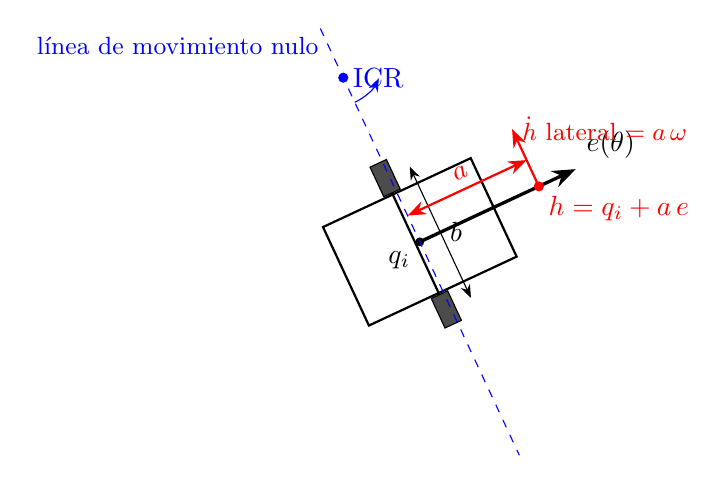
\begin{tikzpicture}[scale=1.15,>=Stealth]
  % chasis
  \draw[thick,rotate=25] (-0.9,-0.6) rectangle (0.9,0.6);
  \coordinate (O) at (0,0);
  % eje y ruedas
  \draw[thick,rotate=25] (-0.05,-0.75) -- (-0.05,0.75);
  \draw[fill=black!70,rotate=25] (-0.15,0.62) rectangle (0.05,0.98);
  \draw[fill=black!70,rotate=25] (-0.15,-0.98) rectangle (0.05,-0.62);
  \draw[<->,rotate=25] (0.25,-0.8) -- (0.25,0.8) node[midway,right] {$b$};
  % rumbo e y punto adelantado h
  \draw[->,very thick] (O) -- ++(25:1.9) node[above right] {$e(\theta)$};
  \fill (O) circle (1.4pt) node[below left] {$q_i$};
  \coordinate (H) at ($(O)+(25:1.45)$);
  \fill[red] (H) circle (1.6pt) node[below right] {$h=q_i+a\,e$};
  \draw[red,thick,<->] ($(O)+(115:0.32)$) -- ($(H)+(115:0.32)$) node[midway,above,sloped] {$a$};
  % linea de movimiento nulo (perpendicular al rumbo por el eje)
  \draw[dashed,blue] ($(O)+(115:2.6)$) -- ($(O)+(-65:2.6)$) node[pos=0.04,left,blue] {\small l\'inea de movimiento nulo};
  % ICR sobre esa linea
  \coordinate (ICR) at ($(O)+(115:2.0)$);
  \fill[blue] (ICR) circle (1.6pt) node[right,blue] {ICR};
  \draw[blue,->,thin] (ICR) ++(-65:0.3) arc (-65:-25:0.55);
  % velocidad lateral admisible en h
  \draw[->,red,thick] (H) -- ++(115:0.7) node[right] {\small $\dot h$ lateral $=a\,\omega$};
\end{tikzpicture}
\caption{AMR diferencial: dos ruedas fijas sobre un mismo eje ($\delta_m=2$, $\delta_s=0$), rumbo $e$, punto de contacto adelantado $h=q_i+a\,e$. La línea de movimiento nulo es la perpendicular al rumbo por el eje; el ICR es libre sobre ella. El centro del eje no puede moverse lateralmente, pero $h$ sí, a razón $a\,\omega$: es \cref{pr:fuera-eje}.}
\label{fig:amr}
\end{figure}}

% ---------- 2. Carga con contactos, normales, conos de friccion; cargo vs caging
\newcommand{\figCarga}{%
\begin{figure}[!ht]\centering
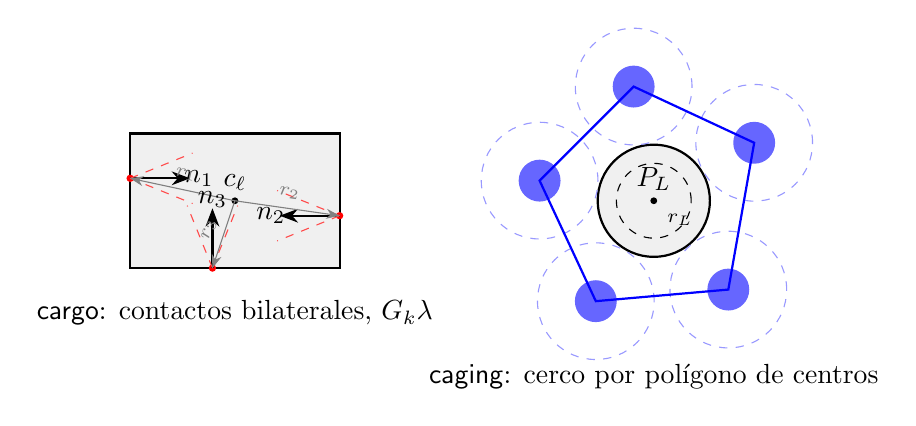
\begin{tikzpicture}[scale=0.95,>=Stealth]
  \begin{scope}
    \draw[thick,fill=black!6] (-1.4,-0.9) rectangle (1.4,0.9);
    \fill (0,0) circle (1.3pt) node[above] {$c_\ell$};
    \foreach \x/\y/\ang/\n in {-1.4/0.3/0/1, 1.4/-0.2/180/2, -0.3/-0.9/90/3}{
      \coordinate (P\n) at (\x,\y);
      \fill[red] (P\n) circle (1.4pt);
      \draw[->,thick] (P\n) -- ++(\ang:0.8) node[pos=1.15] {$n_\n$};
      \draw[dashed,red!70] (P\n) -- ++(\ang+22:0.9); \draw[dashed,red!70] (P\n) -- ++(\ang-22:0.9);
      \draw[->,gray] (0,0) -- (P\n) node[midway,sloped,above,gray] {\scriptsize $r_\n$};
    }
    \node at (0,-1.5) {\textsf{cargo}: contactos bilaterales, $G_k\bm\lambda$};
  \end{scope}
  \begin{scope}[xshift=5.6cm]
    \draw[thick,fill=black!6] (0,0) circle (0.75);
    \fill (0,0) circle (1.3pt) node[above] {$P_L$};
    \draw[dashed] (0,0) circle (0.5) node[below right=2pt] {\scriptsize $r_L$};
    \foreach \a in {30,100,170,240,310}{
      \fill[blue!60] (\a:1.55) circle (0.28);
      \draw[blue!40,dashed] (\a:1.55) circle (0.28+0.5);
    }
    \draw[blue,thick] (30:1.55) -- (100:1.55) -- (170:1.55) -- (240:1.55) -- (310:1.55) -- cycle;
    \node at (0,-2.35) {\textsf{caging}: cerco por polígono de centros};
  \end{scope}
\end{tikzpicture}
\caption{Los dos modos. Izquierda: en \textsf{cargo} cada puesto fija un punto $p_{ks}$, una normal $n_{ks}$ y un cono de fricción; el brazo $r_i$ decide el par, no solo la fuerza (\cref{obs:brazo}). Derecha: en \textsf{caging} no hay agarre; la carga (disco inscrito $r_L$) no puede escapar si los discos prohibidos (radio $r_i+r_L$) cubren el polígono de centros, \cref{th:cerco}.}
\label{fig:carga}
\end{figure}}

% ---------- 3. Disco de friccion compartido por rueda
\newcommand{\figDisco}{%
\begin{figure}[!ht]\centering
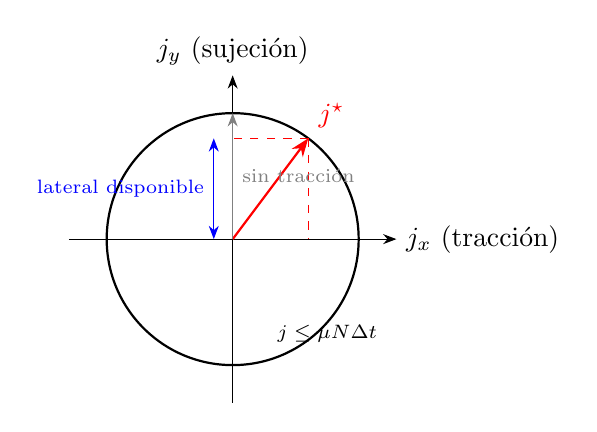
\begin{tikzpicture}[scale=1.6,>=Stealth]
  \draw[thick] (0,0) circle (1);
  \draw[->] (-1.3,0) -- (1.3,0) node[right] {$j_x$ (tracción)};
  \draw[->] (0,-1.3) -- (0,1.3) node[above] {$j_y$ (sujeción)};
  \node at (0.75,-0.75) {\scriptsize $\lVert j\rVert\le\mu N\Delta t$};
  \draw[->,red,thick] (0,0) -- (0.60,0.80) node[above right] {$j^\star$};
  \draw[dashed,red] (0.60,0.80) -- (0.60,0); \draw[dashed,red] (0.60,0.80) -- (0,0.80);
  \draw[<->,blue] (-0.15,0) -- (-0.15,0.80) node[midway,left,blue] {\scriptsize lateral disponible};
  \draw[->,gray] (0,0) -- (0,1) node[pos=0.5,right,gray] {\scriptsize sin tracción};
\end{tikzpicture}
\caption{Un solo disco de Coulomb por rueda: tracción longitudinal y reacción lateral comparten el presupuesto $\mu N\Delta t$. Cuanta más tracción se pide, menos sujeción queda, \cref{pr:disco-friccion}.}
\label{fig:disco}
\end{figure}}

% ---------- 4. Automata de mision con conjuntos anidados
\newcommand{\figAutomata}{%
\begin{figure}[!ht]\centering
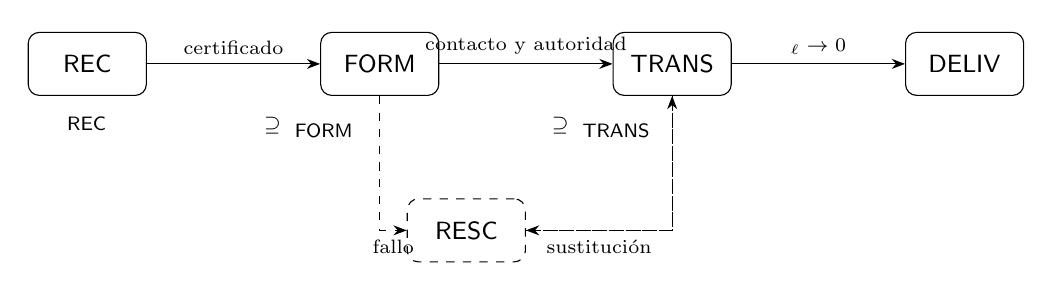
\begin{tikzpicture}[>=Stealth,node distance=2.2cm,every node/.style={font=\small}]
  \node[draw,rounded corners,minimum width=1.5cm,minimum height=0.8cm] (REC) {\textsf{REC}};
  \node[draw,rounded corners,minimum width=1.5cm,minimum height=0.8cm,right=of REC] (FORM) {\textsf{FORM}};
  \node[draw,rounded corners,minimum width=1.5cm,minimum height=0.8cm,right=of FORM] (TRANS) {\textsf{TRANS}};
  \node[draw,rounded corners,minimum width=1.5cm,minimum height=0.8cm,right=of TRANS] (DELIV) {\textsf{DELIV}};
  \node[draw,rounded corners,dashed,minimum width=1.5cm,minimum height=0.8cm,below=1.3cm of FORM,xshift=1.1cm] (RESC) {\textsf{RESC}};
  \draw[->] (REC) -- node[above] {\scriptsize certificado} (FORM);
  \draw[->] (FORM) -- node[above] {\scriptsize contacto y autoridad} (TRANS);
  \draw[->] (TRANS) -- node[above] {\scriptsize $\Wdem_\ell\to0$} (DELIV);
  \draw[->,dashed] (FORM) |- node[pos=0.75,below] {\scriptsize fallo} (RESC);
  \draw[->,dashed] (TRANS) |- (RESC);
  \draw[->,dashed] (RESC) -| node[pos=0.25,below] {\scriptsize sustitución} (TRANS);
  \node[below=0.15cm of REC] {\scriptsize $\Kcal_{\textsf{REC}}$};
  \node[below=0.15cm of FORM,xshift=-0.9cm] {\scriptsize $\supseteq\ \Kcal_{\textsf{FORM}}$};
  \node[below=0.15cm of TRANS,xshift=-0.9cm] {\scriptsize $\supseteq\ \Kcal_{\textsf{TRANS}}$};
\end{tikzpicture}
\caption{Autómata de misión (\cref{def:automata}). Avanzar de fase es entrar en un conjunto admisible más pequeño (\cref{pr:anidados}); la guarda \textsf{REC}$\to$\textsf{FORM} es también el compromiso conjunto que descarta el mal equilibrio (\cref{obs:guarda-fuerte}).}
\label{fig:automata}
\end{figure}}

% ---------- 5. Lazo EDM-PDM: decisiones, pagos, multiplicadores, signo negativo
\newcommand{\figLazo}{%
\begin{figure}[!ht]\centering
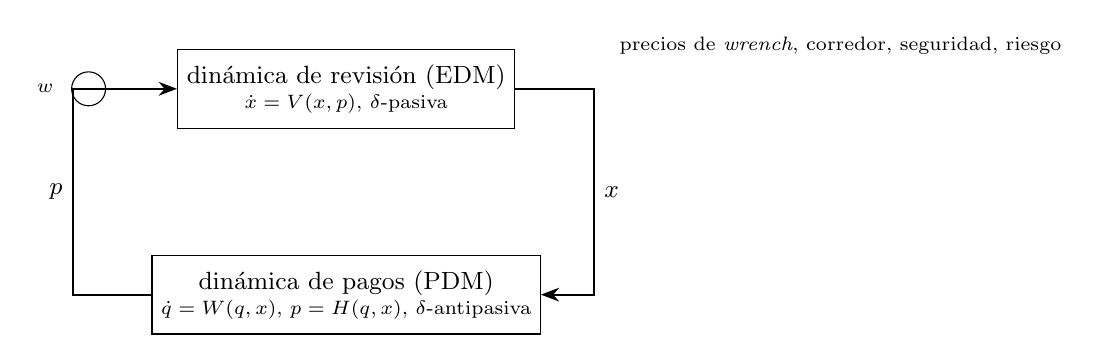
\begin{tikzpicture}[>=Stealth,every node/.style={font=\small},node distance=1.6cm]
  \node[draw,minimum width=3.6cm,minimum height=1cm,align=center] (EDM) {dinámica de revisión (EDM)\\[-2pt]\scriptsize $\dot x=V(x,p)$, $\delta$-pasiva};
  \node[draw,minimum width=3.6cm,minimum height=1cm,align=center,below=of EDM] (PDM) {dinámica de pagos (PDM)\\[-2pt]\scriptsize $\dot q=W(q,x)$, $p=H(q,x)$, $\delta$-antipasiva};
  \draw[->,thick] (EDM.east) -- ++(1.0,0) |- node[pos=0.25,right] {$x$} (PDM.east);
  \draw[->,thick] (PDM.west) -- ++(-1.0,0) |- node[pos=0.25,left] {$p$} (EDM.west);
  \node[draw,circle,inner sep=1pt,left=0.35cm of EDM.west,xshift=-0.55cm] (S) {$-$};
  \node[left=0.1cm of S] {\scriptsize $w$};
  \node[right=1.2cm of EDM.east,yshift=0.55cm] {\scriptsize precios de \emph{wrench}, corredor, seguridad, riesgo};
\end{tikzpicture}
\caption{Interconexión EDM--PDM. El signo negativo de la realimentación es lo que convierte un bloque $\delta$-pasivo en $\delta$-antipasivo con el mismo $\sigma$ (\cref{pr:composiciones}); el reposo es $p^\star=(H+\tfrac{d_p}{\alpha}I)^{-1}w$ con error de vaciado $\tfrac{d_p}{\alpha}p^\star$ (\cref{th:N-precios}).}
\label{fig:lazo}
\end{figure}}

% ---------- 6. Jerarquia de grafos de proximidad
\newcommand{\figGrafos}{%
\begin{figure}[!ht]\centering
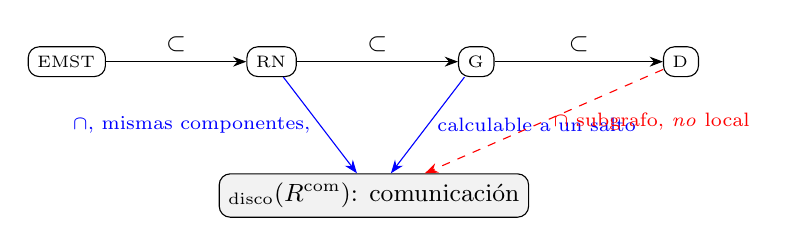
\begin{tikzpicture}[>=Stealth,every node/.style={font=\small}]
  \node[draw,rounded corners] (E) at (0,0) {$\Gcal_{\mathrm{EMST}}$};
  \node[draw,rounded corners] (R) at (2.6,0) {$\Gcal_{\mathrm{RN}}$};
  \node[draw,rounded corners] (G) at (5.2,0) {$\Gcal_{\mathrm{G}}$};
  \node[draw,rounded corners] (D) at (7.8,0) {$\Gcal_{\mathrm{D}}$};
  \draw[->] (E) -- node[above] {$\subset$} (R); \draw[->] (R) -- node[above] {$\subset$} (G); \draw[->] (G) -- node[above] {$\subset$} (D);
  \node[draw,rounded corners,fill=black!5] (disk) at (3.9,-1.7) {$\Gcal_{\mathrm{disco}}(R^{\mathrm{com}})$: comunicación};
  \draw[->,blue] (R) -- node[left,blue] {\scriptsize $\cap$, mismas componentes,} (disk);
  \draw[->,blue] (G) -- node[right,blue] {\scriptsize calculable a un salto} (disk);
  \draw[->,red,dashed] (D) -- node[right,red] {\scriptsize $\cap$ subgrafo, \emph{no} local} (disk);
\end{tikzpicture}
\caption{Orden de los grafos de proximidad (\cref{th:jerarquia-grafos}). Gabriel y vecindad relativa cortados al disco conservan exactamente las componentes conexas y se calculan con un salto; Delaunay cortado al disco no es localmente calculable. El adelgazamiento actúa solo sobre el grafo de comunicación (\cref{obs:cuatro-grafos}).}
\label{fig:grafos}
\end{figure}}

% ---------- 7. Caza del ciervo: creencia critica p*(r*)
\newcommand{\figCiervo}{%
\begin{figure}[!ht]\centering
\begin{tikzpicture}[scale=1.0,>=Stealth]
  \draw[->] (0,0) -- (9.6,0) node[right] {$r^\star$};
  \draw[->] (0,0) -- (0,4.2) node[above] {$p^\star$};
  \foreach \r/\p in {2/0.045,3/0.123,4/0.205,5/0.290,6/0.376,7/0.463,8/0.551,9/0.641,10/0.732}{
    \fill (\r,{\p*5}) circle (1.6pt);
    \node[below] at (\r,0) {\scriptsize \r};
  }
  \draw[thick,blue] plot coordinates {(2,0.225) (3,0.615) (4,1.025) (5,1.45) (6,1.88) (7,2.315) (8,2.755) (9,3.205) (10,3.66)};
  \draw[dashed,red] plot coordinates {(2,0.16) (3,0.56) (4,0.985) (5,1.42) (6,1.86) (7,2.31) (8,2.765) (9,3.225) (10,3.695)};
  \foreach \y in {0.2,0.4,0.6}{ \draw (0,{\y*5}) -- (-0.1,{\y*5}) node[left] {\scriptsize \y}; }
  \node[blue] at (4.2,3.2) {\scriptsize exacto (binomial)};
  \node[red] at (7.6,1.1) {\scriptsize aproximación normal};
\end{tikzpicture}
\caption{Creencia crítica de la caza del ciervo para $n=12$, $B=10$, $c=1$, $w=3$ (\cref{th:N-ciervo}): la cuenca de la cooperación $1-p^\star$ cae de $0{,}955$ a $0{,}268$ al crecer la coalición exigida. La aproximación normal difiere en menos de $0{,}013$.}
\label{fig:ciervo}
\end{figure}}
